\subsection{Estudo geométrico}\label{sec::estudo_geom}
O estudo geométrico é uma avaliação simples de alcance dos manipuladores
industriais no ambiente do aro câmara. Tem como objetivo verificar se o
manipulador consegue percorrer todos os pontos da pá dentro das restrições da
tarefa HVOF, assumindo a pá planar, e diferentes posições de base. O estudo
leva em consideração as seguintes posições para o manipulador: escotilha
superior e base móvel; manipulador em frente à pá e base móvel verticalmente;
manipulador entre as pás e base móvel verticalmente.

Assumimos $R = 3.95 m$ e $R_m = 3 m$, onde $R$ é a distância do centro do cone à
superfície do aro câmara, e $R_m$ é o comprimento da pá. Logo, podemos
inferir o comprimento do aro câmara $P = 2*\pi *R = 24.81 m$. Em relação ao
centro do cone, o setor circular que cada pá ocupa tem um ângulo, em radianos,
de $\beta = \frac{R_m*2*\pi}{P} = 0.76$, e a metade do setor circular entre
as pás tem ângulo $\alpha = \pi/4$, já que elas são simetricamente distribuídas.
A figura~\ref{pa} mostra os parâmetros acima, onde as pás estão representadas
como setores circulares roxos e metade da distância entre as pás como setor
azul.

\begin{figure}[h!]
\centering
	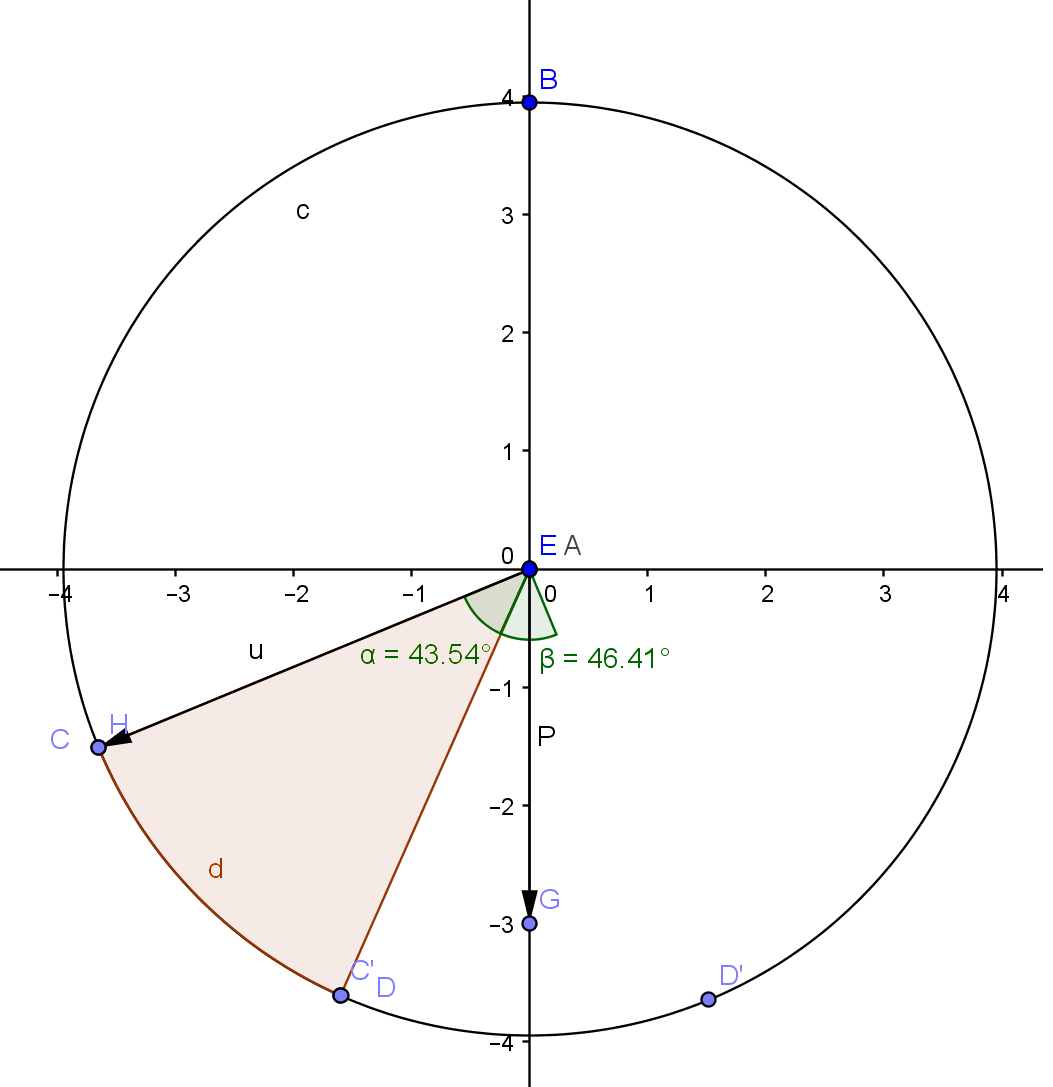
\includegraphics[width=\columnwidth]{figs/estudo/geometrico/pa.png} 
	\caption{Parâmetros do aro câmara.}
	\label{pa}
\end{figure}

Utilizando notação vetorial, temos: $\overrightarrow{P_1} = (0,-R,0)$. Considere
$$\overrightarrow{{P_2}} = R_z(-(\beta/2 + \alpha))
\overrightarrow{P_1}$$ e $$\overrightarrow{{P_3}} = R_z(-\alpha))
\overrightarrow{P_1}$$ , onde $R_z$ é rotação em  torno de $Z$. Considere agora
o vetor $$\overrightarrow{d} =
R_{\overrightarrow{\overline{P_3}}}(-\omega)R_z(-\beta/2 -
\alpha)\overrightarrow{P_1}$$, onde $R_{\overrightarrow{\overline{P_3}}}$ é rotação em torno do vetor unitário
na direção de $\overrightarrow{P_3}$ e $\omega$ é o ângulo de rotação da pá em
seu próprio eixo (valor que pode variar de $0$ a $28^o$).
Dessa forma, busca-se o $$min (\left \| \overrightarrow{d} - \overrightarrow{M} 
\right \|) =\left \| R_{\overrightarrow{\overline{P_3}}}(-\omega)R_z(-\beta/2 -
\alpha)\overrightarrow{P} - \overrightarrow{M} \right \|$$, onde
$\overrightarrow{M}=(0,-x,0)$ é a localização da base do manipulador. Dessa
forma, obtemos a menor distância entre base e o extremo da pá para $\omega,
x, \alpha$. Consequentemente, pode-se inferir o alcance mínimo do manipulador.

Pode-se posicionar a base do manipulador em diferentes valores de $\alpha$, que é
o mesmo que girar a turbina e alterar a posição da pá. Para $\alpha = 0$, por
exemplo, o manipulador se encontra em frente à pá, e para $\alpha = \pi/4$ ele está entre as pás.

A análise para a escotilha inferior consiste em posicionar o manipulador no
centro ou entre as pás ($\alpha = 0$ ou $\alpha = \pi/4$) e assumir $\omega =
\pi/4$ (pá girada $45^o$). No caso em que o
manipulador se encontra em frente à pá, alcançar todos os pontos da pá  é
traçar uma circunferência que a envolve, representando
a área de alcance do manipulador. Após o cálculo desta
circunferência, deve-se distanciar ortogonalmente a base do manipulador à pá,
pois este deve estar posicionado de uma maneira que não haja colisões. A
figura~\ref{paemfrente} mostra a circunferência, cujo raio pode ser encontrado
analiticamente pelas equações:
$$\rho ^2 = r^2+R_c^2-2R_crcos(\beta)$$
$$\rho ^2 = R^2+R_c^2-2R_cRcos(\beta)$$
onde $R$ é o raio do aro câmara, $r$ é o raio do cone da turbina, $R_c$ é a
distância do centro da pá ao centro do cone e $\rho$ é o raio da circunferência
que circunscreve a pá. Obtêm-se  $\rho=1.6387$ e $h=1.0157$, onde $h$ é a altura
da base do manipulador ($R-R_c$). Observe que $\rho$ é o alcance para o
manipulador sob a pá, logo temos que supor uma distância $d$ entre o manipulador
e a pá a fim de evitar colisões. Assumindo diversos valores para $d$, obtemos o
gráfico~\ref{reach} que mostra o alcance necessário do manipulador versus
distância que ele se encontra da pá. 

\begin{figure}[h!]
\centering
	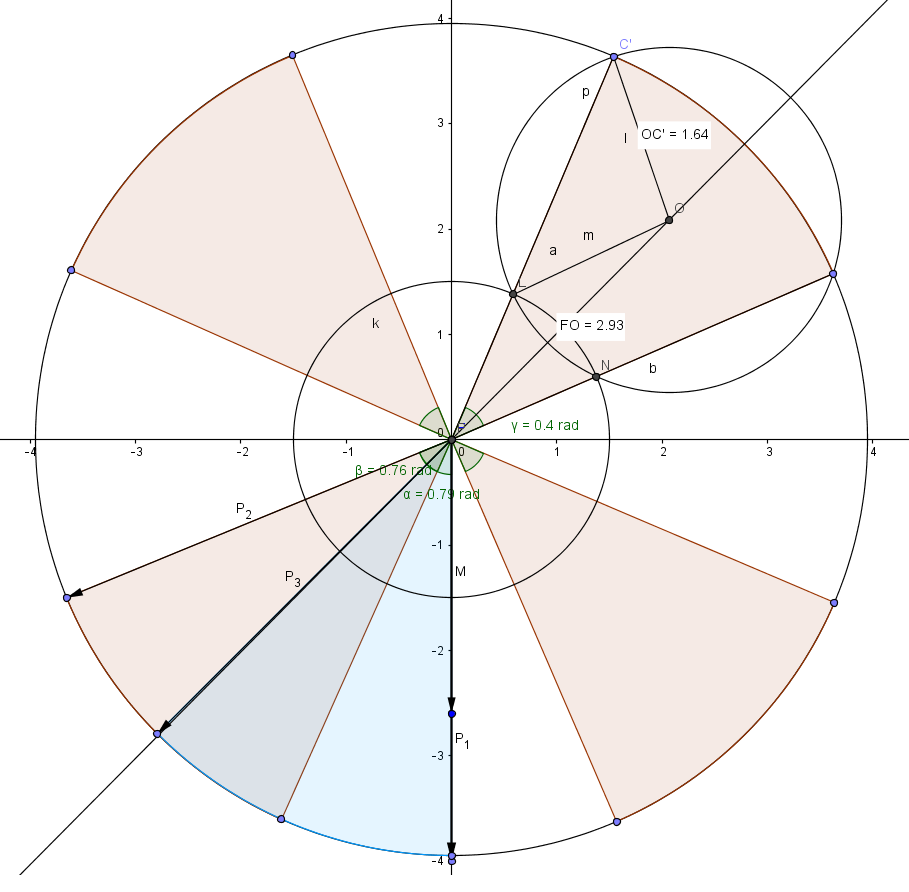
\includegraphics[width=\columnwidth]{figs/estudo/geometrico/paemfrente.png} 
	\caption{Estudo geométrico do manipulador industrial em frente à pá.}
	\label{paemfrente}
\end{figure}

\begin{figure}[h!]
\centering
	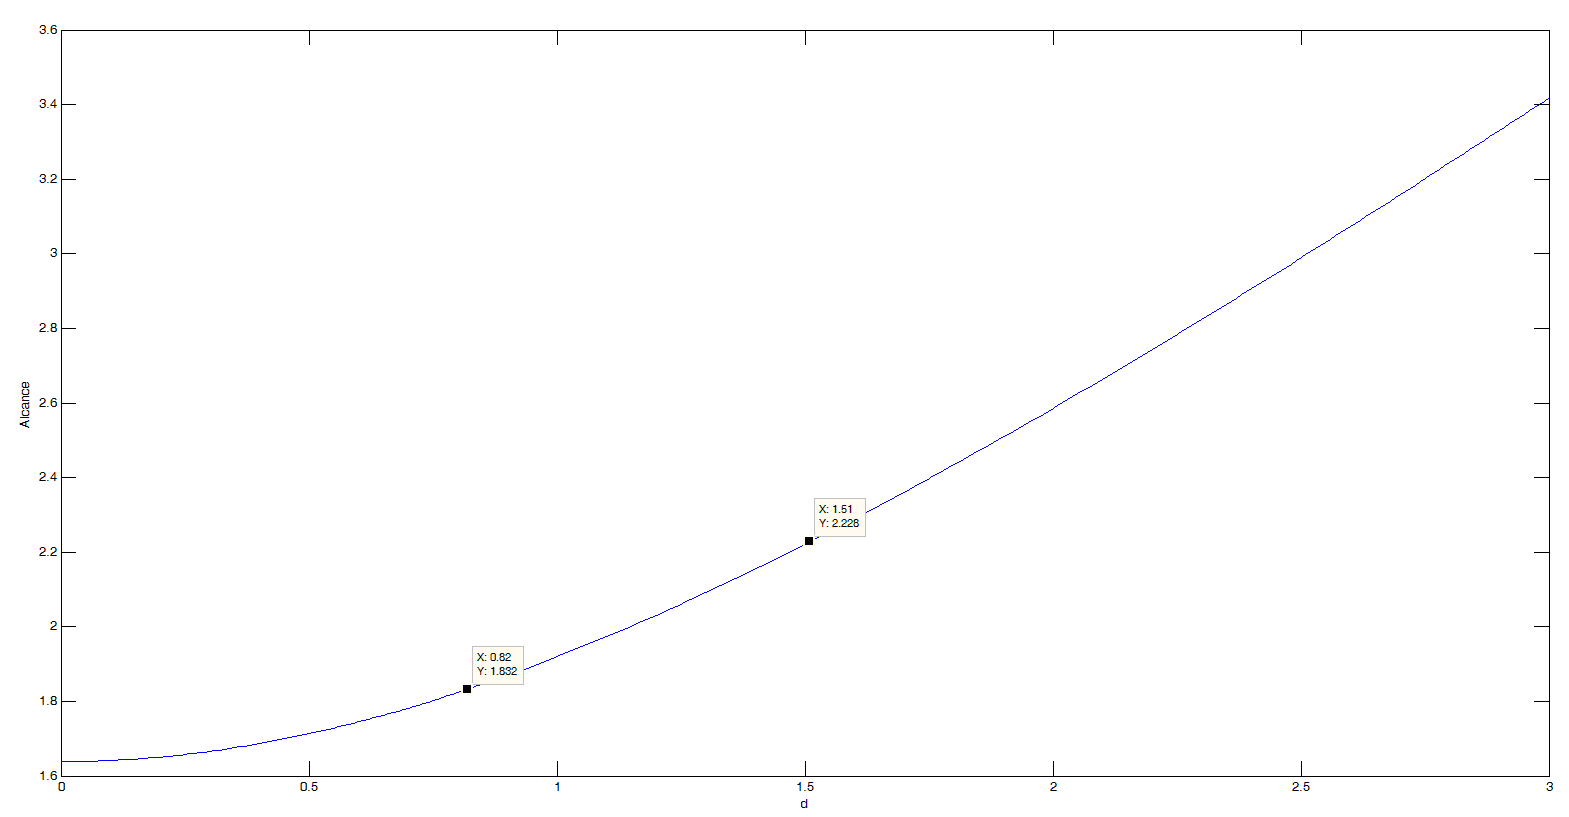
\includegraphics[width=\columnwidth]{figs/estudo/geometrico/reach.png} 
	\caption{Gráfico que mostra o alcance necessário do manipulador versus a
	distância que ele se encontra da pá.}
	\label{reach} 
\end{figure}

Para uma posição fixa da base, o manipulador, a uma distância de 1 m
da pá, necessita ter alcance máximo de 1.7 m para percorrer todos os pontos, se
considerarmos os 230 mm de distância mínimo entre pá e pistola. Esta é uma
solução inviável para um manipulador de médio porte e com o payload necessário.
Portanto, será realizada uma análise mais profunda levando em consideração
possibilidade de movimentação da base horizontalmente por atuador ou
manualmente.

Na escotilha superior, como há restrição em relação ao manipulador (LBR 820), há
a necessidade de uma base móvel, que possa assumir diversos comprimentos e
posições. A solução de uma base com dois elos está representada na
figura~\ref{pakuka}, onde os elos i e j estão representados em verde, o cone
da turbina representado pela circunferência c, o espaço de trabalho planar do
manipulador está representado em verde, e a pá representada como um setor
circular em vermelho.

\begin{figure}[h!]
\centering
	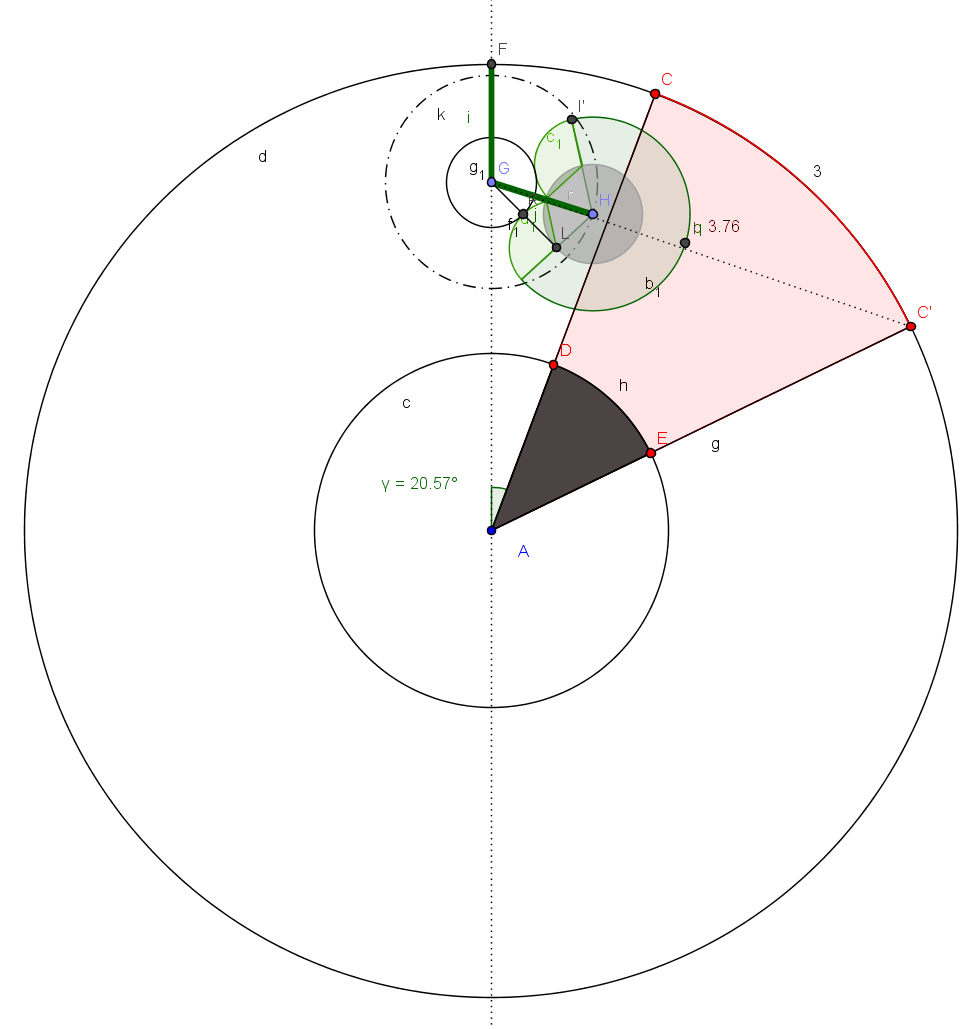
\includegraphics[width=\columnwidth]{figs/estudo/geometrico/kuka.png} 
	\caption{Estudo geométrico do manipulador industrial Kuka 820 na escotilha
	superior e base de dois elos.}
	\label{pakuka}
\end{figure}

A análise puramente geométrica não considera o formato real curvilíneo da pá e
é apenas uma análise de alcance de extremos. Isso não garante que a área de
trabalho do manipulador cubra todos os pontos da pá e ainda não considera
possíveis colisões com o ambiente e/ou própria base e manipulador. O estudo do
espaço de trabalho por simulações se faz necessário para garantir a viabilidade
dos manipuladores industriais.
